\begin{enumerate}[label=\thechapter.\arabic*,ref=\thechapter.\theenumi]
\item The network shown below has a resonant frequency of 150 kHz and bandwidth of 600
Hz. The Q-factor of the network is \rule{1cm}{0.15mm}\\
(rounded off to one decimal place).\\
\hfill(GATE 2022 EC)\\
\begin{figure}[ht]
  \centering
  
      \begin{circuitikz}[american]
\draw (0,3) to [short,*-, i=$i_c$] (1,3) to [R=$R$] (4,3);
\draw (0,0) to [short, *-] (4,0);
\draw (4,3) to [short, i=$i_d$] (4,2.5) to [C=$C$] (4,0);
\end{circuitikz}
  
  \caption{Circuit 1}
\end{figure}\\
\solution\\
\iffalse
\let\negmedspace\undefined
\let\negthickspace\undefined
\documentclass[journal,12pt,twocolumn]{IEEEtran}
\usepackage{cite}
\usepackage{amsmath,amssymb,amsfonts,amsthm}
\usepackage{algorithmic}
\usepackage{graphicx}
\usepackage{textcomp}
\usepackage{xcolor}
\usepackage{txfonts}
\usepackage{listings}
\usepackage{enumitem}
\usepackage{mathtools}
\usepackage{gensymb}
\usepackage{comment}
\usepackage[breaklinks=true]{hyperref}
\usepackage{tkz-euclide} 
\usepackage{listings}
\usepackage{gvv}                                        
\def\inputGnumericTable{}                                 
\usepackage[latin1]{inputenc}                                
\usepackage{color}                                            
\usepackage{array}                                            
\usepackage{longtable}                                       
\usepackage{calc}                                             
\usepackage{multirow}                                         
\usepackage{hhline}                                           
\usepackage{ifthen}                                           
\usepackage{lscape}
\usepackage[center]{caption} % center the captions to figure

\newtheorem{theorem}{Theorem}[section]
\newtheorem{problem}{Problem}
\newtheorem{proposition}{Proposition}[section]
\newtheorem{lemma}{Lemma}[section]
\newtheorem{corollary}[theorem]{Corollary}
\newtheorem{example}{Example}[section]
\newtheorem{definition}[problem]{Definition}
\newcommand{\BEQA}{\begin{eqnarray}}
\newcommand{\EEQA}{\end{eqnarray}}
\newcommand{\define}{\stackrel{\triangle}{=}}
\theoremstyle{remark}
\newtheorem{rem}{Remark}
\begin{document}

\newcolumntype{M}[1]{>{\centering\arraybackslash}m{#1}}
\newcolumntype{N}{@{}m{0pt}@{}}

\bibliographystyle{IEEEtran}
\vspace{3cm}

\title{GATE 2022 BM 14 Q} 
\author{ee23btech11223 - Soham Prabhakar More% <-this % stops a space
}
\maketitle
\newpage
\bigskip

\renewcommand{\thefigure}{\theenumi}
\renewcommand{\thetable}{\theenumi}

\bibliographystyle{IEEEtran}

\textbf{Question:} $x\brak{t}$ is a real continuous-time signal whose magnitude frequency response
$\abs{X\brak{j\Omega}}$ is shown below. After sampling $x\brak{t}$ at 100 $rad.s^{-1}$, the spectral point P
is down-converted to \rule{1cm}{0.15mm} $rad.s^{-1}$ in the spectrum of the sampled signal.
\hfill{(GATE 2022 BM 14 Q)}
\begin{figure}[h!]
    \renewcommand\thefigure{1}
    \centering
    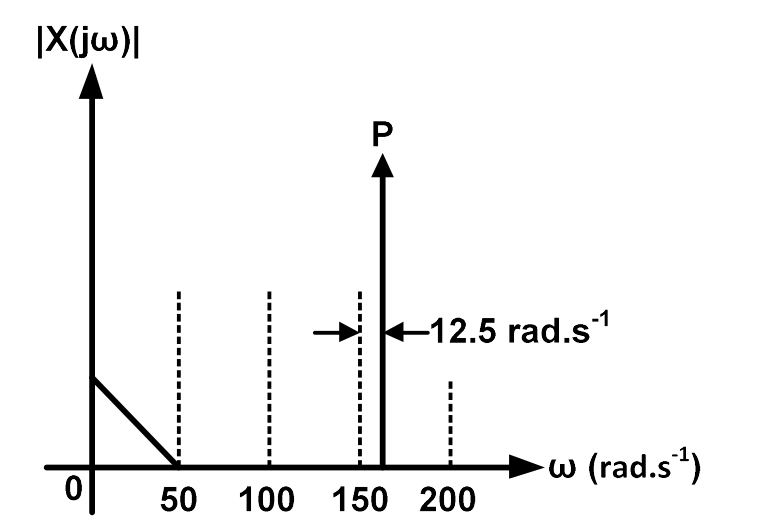
\includegraphics[width=\columnwidth]{2022/BM/14/figs/question.png}
    \caption[short]{Plot of $\abs{X\brak{j\omega}}$}
    \label{fig:2023.bm.14.img1}
\end{figure}

\solution
\fi
\begin{table}[ht]
    \renewcommand\thetable{1}
\begin{tabular}{|c|c|}
    \hline 
    \textbf{Parameter}&\textbf{Description} \\
    \hline
    $w\brak{t}$ & Sampling Function \\
    \hline
	$W\brak{j\omega}$ & Fourier Transform of $w\brak{t}$ \\
    \hline
    $x\brak{t}$ & Input Signal \\
    \hline
    $X\brak{j\omega}$ & Input Signal Frequency Spectrum \\
    \hline
    $x_s\brak{t}$ & Sampled Input Signal \\
    \hline
    $X_s\brak{j\omega}$ & Sampled Signal Frequency Spectrum \\
    \hline
\end{tabular}

\caption{Table of parameters}
\label{Table:1}


\end{table} \\
The sampling function is:
\begin{align}
    w(t) &= \sum_{k = -\infty}^{\infty}\delta\brak{t - \frac{2\pi k}{100}} \\
    W(j\omega) &= 100\sum_{k = -\infty}^{\infty}\delta\brak{j\brak{\omega - 100k}}
\end{align}
then the sampled function: 
\begin{align}
    x_s\brak{t} &= x\brak{t}w\brak{t} \\
    X_s\brak{j\omega} &= X\brak{j\omega} * W\brak{j\omega} \\
    X_s\brak{j\omega} &= \int_{-\infty}^{\infty}X\brak{j\theta}W\brak{j\brak{\omega - \theta}}d\theta \\
    X_s\brak{j\omega} &= 100\sum_{k = -\infty}^{\infty}\int_{-\infty}^{\infty}X\brak{j\theta}\delta\brak{j\brak{\omega - 100k - \theta}}d\theta \\
    X_s\brak{j\omega} &= 100\sum_{k = -\infty}^{\infty}X\brak{j\brak{\omega - 100k}} 
\end{align}
Thus, The down sampled point is at:
\begin{align}
    \omega &= \abs{162.5 - 100k}
\end{align}
where $k$ is the nearest integer to $\frac{162.5}{100}$, which is 2\\
Thus,
\begin{align}
    \omega = 37.5\,rad\,s^{-1}
\end{align}

\begin{figure}[h!]
    \renewcommand\thefigure{2}
    \centering
    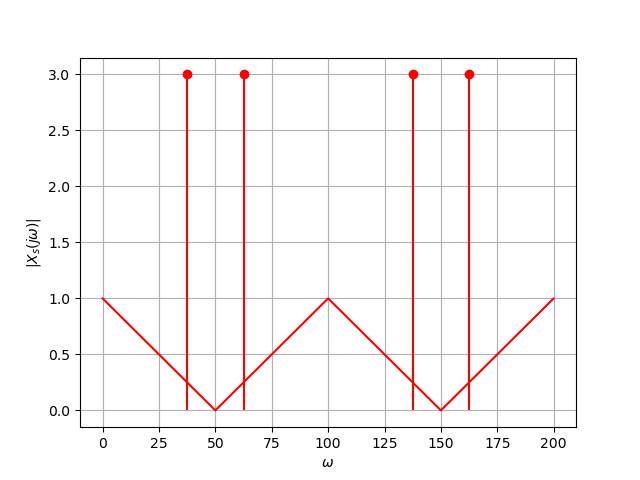
\includegraphics[width=\columnwidth]{2022/BM/14/figs/X_s.png}
    \caption[short]{Plot of $\abs{X_s\brak{j\omega}}$}
    \label{fig:2023.bm.14.img2}
\end{figure}

%\end{document}

\pagebreak
\item For the circuit shown, the locus of the impedance $ Z\brak{j\omega}$ is plotted as $ \omega$ increases from zero to infinity. The values of $ R_1$ and $ R_2$ are:
\begin{enumerate}
    \item[(A)] $ R_1 = 2\text{ k\ohm}, R_2 = 3\text{ k\ohm}$
    \item[(B)]$ R_1 = 5\text{ k\ohm}, R_2 = 2\text{ k\ohm}$
    \item[(C)] $ R_1 = 5\text{ k\ohm}, R_2 = 2.5\text{ k\ohm}$
    \item[(D)] $ R_1 = 2\text{ k\ohm}, R_2 = 5\text{ k\ohm}$
\end{enumerate}

\begin{figure}[h!]
    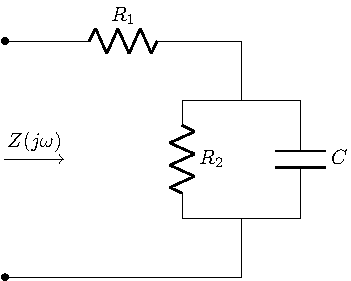
\includegraphics[width = 0.6\columnwidth]{2022/EC/38/figs/qn_fig.pdf}
    \caption{Figure of circuit}
    \centering
    \label{fig: ece38_qn_fig}
\end{figure}

\begin{figure}[h!]
    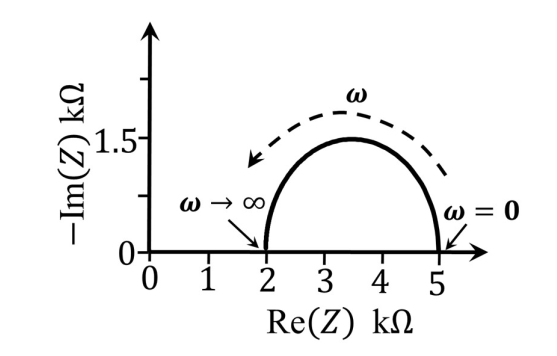
\includegraphics[width = 0.6\columnwidth]{2022/EC/38/figs/fig_2.png}
    \caption{}
    \centering
    \label{fig: ece38qn_2_fig}
\end{figure}
\hfill(GATE ECE 2022)\\
\solution
 \iffalse
\let\negmedspace\undefined
\let\negthickspace\undefined
\documentclass[journal,12pt,twocolumn]{IEEEtran}
\usepackage{cite}
\usepackage{amsmath,amssymb,amsfonts,amsthm}
\usepackage{algorithmic}
\usepackage{graphicx}
\usepackage{textcomp}
\usepackage{xcolor}
\usepackage{txfonts}
\usepackage{listings}
\usepackage{enumitem}
\usepackage{mathtools}
\usepackage{gensymb}
\usepackage{comment}
\usepackage[breaklinks=true]{hyperref}
\usepackage{tkz-euclide}
\usepackage{listings}
\usepackage{gvv}
\def\inputGnumericTable{}
\usepackage[latin1]{inputenc}
\usepackage{color}
\usepackage{array}
\usepackage{longtable}
\usepackage{calc}
\usepackage{multirow}
\usepackage{hhline}
\usepackage{ifthen}
\usepackage{lscape}

\newtheorem{theorem}{Theorem}[section]
\newtheorem{problem}{Problem}
\newtheorem{proposition}{Proposition}[section]
\newtheorem{lemma}{Lemma}[section]
\newtheorem{corollary}[theorem]{Corollary}
\newtheorem{example}{Example}[section]
\newtheorem{definition}[problem]{Definition}
\newcommand{\BEQA}{\begin{eqnarray}}
\newcommand{\EEQA}{\end{eqnarray}}
\newcommand{\define}{\stackrel{\triangle}{=}}
\theoremstyle{remark}
\newtheorem{rem}{Remark}
\begin{document}

\bibliographystyle{IEEEtran}
\vspace{3cm}

\title{GATE 2022  -AE 63}
\author{EE23BTECH11057 - Shakunaveti Sai Sri Ram Varun$^{}$% &lt;-this % stops a space
}
\maketitle
\newpage
\bigskip
\vspace{2cm}
\textbf{Question: }
For the circuit shown, the locus of the impedance $ Z\brak{j\omega}$ is plotted as $ \omega$ increases from zero to infinity. The values of $ R_1$ and $ R_2$ are:
\begin{enumerate}
    \item[(A)] $ R_1 = 2\text{ k\ohm}, R_2 = 3\text{ k\ohm}$
    \item[(B)]$ R_1 = 5\text{ k\ohm}, R_2 = 2\text{ k\ohm}$
    \item[(C)] $ R_1 = 5\text{ k\ohm}, R_2 = 2.5\text{ k\ohm}$
    \item[(D)] $ R_1 = 2\text{ k\ohm}, R_2 = 5\text{ k\ohm}$
\end{enumerate}

\begin{figure}[h!]
    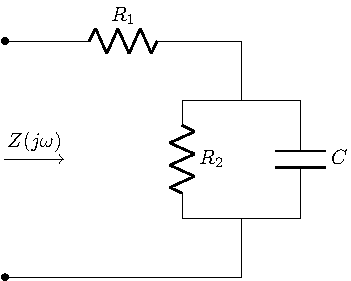
\includegraphics[width = 0.6\columnwidth]{2022/EC/38/figs/qn_fig.pdf}
    \caption{Figure of circuit}
    \centering
    \label{fig: ece38_qn_fig}
\end{figure}

\begin{figure}[h!]
    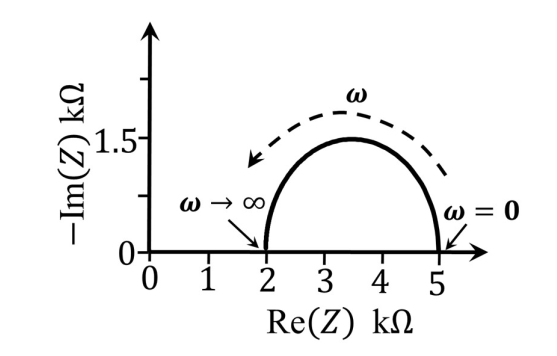
\includegraphics[width = 0.6\columnwidth]{2022/EC/38/figs/fig_2.png}
    \caption{}
    \centering
    \label{fig: ece38qn_2_fig}
\end{figure}
\hfill(GATE ECE 2022 QUESTION 38)\\
\textbf{Solution}:\\
\fi
\begin{table}[h!] 
\centering
\begin{tabular}{|c|c|c|}
    \hline
    \textbf{Parameter} & \textbf{Description} & \textbf{Value} \\
    \hline
    $ Z\brak{j\omega}$ & Impedance of circuit & ? \\
    \hline
    $ R_1$ & Resistor 1  &? \\
    \hline
    $ R_1$ & Resistor 2  &? \\
    \hline
    $ C$ & Capacitor  &? \\
    \hline
    $\omega$ & angular frequency of input voltage& $ \omega$\\
    \hline
\end{tabular}





\caption{input values}
\label{tab: Table2022ECE38}
\end{table}

In $ \omega$ domain (i.e. after Laplace transform) \figref{fig: ece38_qn_fig} can be represented as \figref{fig: ece38_ans_1_fig}
\begin{figure}[h!]
    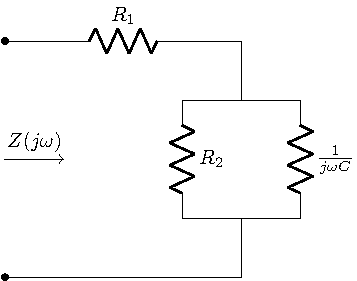
\includegraphics[width = 0.6\columnwidth]{2022/EC/38/figs/answer_fig.pdf}
    \caption{}
    \centering
    \label{fig: ece38_ans_1_fig}
\end{figure}
So, the impedance for the circuit in $ \omega$ domain is:
\begin{align}
Z\brak{j \omega} &= R_1 +  \frac{1}{\frac{1}{R_2}+ j\omega C} \label{eq: ece38_1}
\end{align}
From \figref{fig: ece38qn_2_fig}, $ Z\brak{j\omega}=2$ as $ \omega \to \infty$ and 
$ Z\brak{j\omega}=5$ as $ \omega \to 0$
\begin{align}
2 &= R_1 + \lim_{\omega\to\infty}\frac{1}{\frac{1}{R_2}+ j\omega C}\\
\implies 2 &= R_1 + \lim_{\omega\to\infty}\frac{\frac{1}{R_2}- j \omega C}{\brak{\frac{1}{R_2}}^2+ \brak{\omega C}^2}\\
\implies 2 &= R_1 + \lim_{\omega\to\infty}\frac{\frac{1}{R_2 \omega^2}- j\frac{C}{\omega}}{\brak{\frac{1}{R_2 \omega}}^2+ C^2}\\
\therefore R_1 \label{eq: ece_38_2}&= 2\text{\ohm}\\
5 &= R_1 + \frac{1}{\frac{1}{R_2}+j\brak{0}}\\
\implies 5 &= R_1 + R_2\\
\therefore R_2 &= 3\text{\ohm} 
\end{align}
Hence, option (A) is correct.


\pagebreak
\newpage
\end{enumerate}
